\documentclass[11pt]{article}
\newcommand\tab[1][1cm]{\hspace*{#1}}
\usepackage{graphicx}
\usepackage{float}

\begin{document}
	\title{Ticket Salad Requirements and design document}
	\date{}
	\maketitle
	\tableofcontents
	\newpage
	
	\section{Software architecture overview}
	Figure 1 shows a high-level overview of the software architecture. In particular it shows the decomposition of the system into layers with abstract responsibilities, the core architectural components of the system and the concrete frameworks to be used when realizing these architectural components.
	
	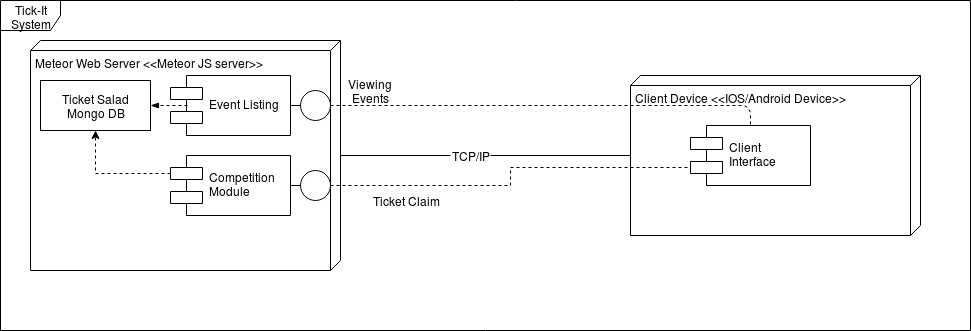
\includegraphics[scale=0.4]{Architecture}
	\caption{Figure 1: }{A high-level overview of the software architecture of the TicketSalad System.}
	
	
	\section{Overall software architecture}
	This section specifies the software architecture requirements and the software architecture design
	for the first level of granularity – the system as a whole. The output will be the high level software
	architecture components, the infrastructure between them and the tactics used at the first level of
	granularity to realize the quality requirements for the system.
	Subsequent sections will focus on the software architecture requirements and design for these
	high-level architectural components. Note that many of the architectural requirements (particularly
	the quality requirements) will be propagated down to lower level architectural components.
	
	\subsection{Architecture requirements}
	\subsubsection{Access and integration requirements}
	This section discusses the software architecture requirements — that is the requirements around the
	software infrastructure within which the application functionality is to be developed. The purpose of this infrastructure is to address the non-functional requirements. In particular, the architecture
	requirements specify
	\begin{itemize}
		\item The architectural responsibilities which need to be addressed.
		\item The access and integration requirements for the system.
		\item The quality requirements
		\item The architecture constraints specified by the client.
	\end{itemize}

	\subsubsection{Quality requirements}
	The quality requirements are the requirements around the quality attributes of the systems and
	the services it provides. This includes requirements like maintainability, flexibility, extensibility,
	performance, scalability, security, auditabilty, usability, and testability requirements.
	\newline
	\newline
	\textbf{2.1.2.1 Flexibility}
	\newline
	\newline
	It is important that the system architecture is such that one can easily
	add different access channels to the system. This is particularly important in the context of the
	proliferation of connected devices in a world transiting to fully embrace the Internet of Things
	(IoT).	
	
	
	Furthermore, persistence architectures and reporting infrastructures are rapidly evolving as can
	be seen from the rapid growth of NoSQL databases, semantic knowledge repositories and big data
	stores. In this context it is important that the application functionality is not locked into any
	specific persistence technology and that one is able to easily modify the persistence provider and
	reporting framework.
	\newline
	\newline
	\textbf{2.1.2.2 Maintainability}
	\newline
	\newline
	Amongst the most important quality requirements for the system is
	\textit{maintainability}. It should be easy to maintain the system in the future. To this end
	\begin{itemize}
		\item Future developers should be able to easily understand the system.
		\item The technologies chosen for the system should be available for a reasonably long time.
		\item Developers should be easily and quickly be able to change aspects of the functionality the system provides.
		\item Developers should be easily and quickly be able to add new functionality to the system.
	\end{itemize}
	\newline
	\newline
	\textbf{2.1.2.3 Scalability}
	\begin{itemize}
		\item Initially the system must be able to support a relatively large group of users, i.e, supporting a maximum of 1000 users.
		\item The architecture of the system should allow for increasing the amount of users to includes several thousands of users.
	\end{itemize}
	\textbf{2.1.2.4 Performance}
	\begin{itemize}
		\item All operations that do not require database communication should respond in less than 0.5 seconds.
		\item All operations that communicate and modify the database should be processed in less than 7 seconds
	\end{itemize}
	The above figures do not include effect of internet speed and device speed have on the system.
	\newline
	\newline
	\textbf{2.1.2.5 Reliability}
	\newline
	\newline
	The system should provide by default a reasonable level of availability and
	reliability and should be deployable within configurations which provide a high level availability, supporting
	\begin{itemize}
		\item Fail-over safety of all components
		\item A deployment without single points failure
		Rapid deployment of new/changing functionality is required for this system.
	\end{itemize}
	\newline
	\newline
	\textbf{2.1.2.6 Security}
	\newline
	\newline
	The system needs to support 
	\begin{itemize}
		\item Login authentication against a NoSQL user repository.
		\item Credit card verification against mastercard and visa repositories.
		\item Payment verification using mastercard and visa services.
	\end{itemize}
	\newline
	\newline
	\textbf{2.1.2.7 Auditability}
	\newline
	\newline
	The system will have a log for all login, logout, bidding and financial transactions, the following will be stored in the log:
	\begin{itemize}
		\item User id
		\item Date/time stamp of the interaction
		\item Response from the interaction
		\item Before and after states of the users profile
	\end{itemize}
	\newline
	\newline
	\textbf{2.1.2.8 Testability}
	\newline
	\newline
	All services offered by the system must be testable through
	\begin{enumerate}
		\item Automated unit tests testing components in isolation using mock objects.
		\item Automated integration tests where components are integrated within the actual environment which test,
		\begin{itemize}
			\item The services are provided if all pre-conditions are met 
			\item That all post conditions hold true after the service is provided
		\end{itemize}
	\end{enumerate}
	\newline
	\newline
	\textbf{2.1.2.9 Usability}
	\newline
	\newline
	
	
	
	
	
	
	
	
	
	
	
	
	
	
	
	
	
	
	
	
	
	
	
	
	
	
	
	
	
	
	\newpage
	\section{Functional Requirements}
	R.1 Ticket Salad shall allow the user to sign up. \newline
	R.1.1Ticket Salad shall allow a user to enter their required information.\newline
	R.1.2 Ticket Salad shall create a user account based on the information.\newline
	R.1.3 Ticket Salad shall reject account creation if the information is not valid.\newline
	R.1.4 Ticket Salad shall secure the account information in secure database.\newline\newline
	R.2 Ticket shall allow the user to Log In\newline
	R.2.1 Ticket Salad shall allow a user to log in to their account.\newline
	R.2.2 Ticket Salad shall allow a user to log out of their account.\newline
	R.2.3Ticket Salad shall reject a login based off invalid details.\newline
	R.2.4 Ticket Salad shall hide all in-app views if a user is logged out.\newline\newline
	R.3 Ticket Salad shall allow the user to view events
	\newline R3.1 Ticket Salad shall allow a user to view all current ticket events.
	\newline R.3.2 Ticket Salad shall allow a user to search through the displayed events.
	\newline R.3.3 Ticket Salad shall display more information in the expanded event.
	\newline R.3.4 Ticket Salad shall allow a user to expand a certain event.
	\newline R.3.5 Ticket Salad shall allow a user to bid on an event from the expanded view.
	\newline R.3.6 Ticket Salad shall allow a user to bid on an event directly from the events view.
	\newline R.3.7 Ticket Salad shall notify users when an event closes
	\newline R.3.8 Ticket Salad shall notify a user if they win an event \newline\newline
	R.4 Ticket Salad shall allow the user to gain access to their profile
	\newline R.4.1 Ticket Salad shall allow a user to view their profile.
	\newline R.4.2 Ticket Salad shall allow a user to edit information regarding their profile.
	\newline R.4.3 Ticket Salad shall allow a user to delete their account at their request.
	\newline R.4.4 Ticket Salad shall reject changes to the user’s profile if the information is invalid.\newline\newline
	R.5 Ticket Salad shall allow the user to access their claim credits
	\newline R.5.1 Ticket Salad shall allow a user to view their claim credit balance.
	\newline R.5.2 Ticket Salad shall allow a user to purchase more claim credits.
	\newline R.5.3 Ticket Salad shall allow a user to claim bids if they possess enough credits.
	\newline R.5.4 Ticket Salad shall deduct claim credits when a user bids on an event
	\newline
	\section{Domain Model}
	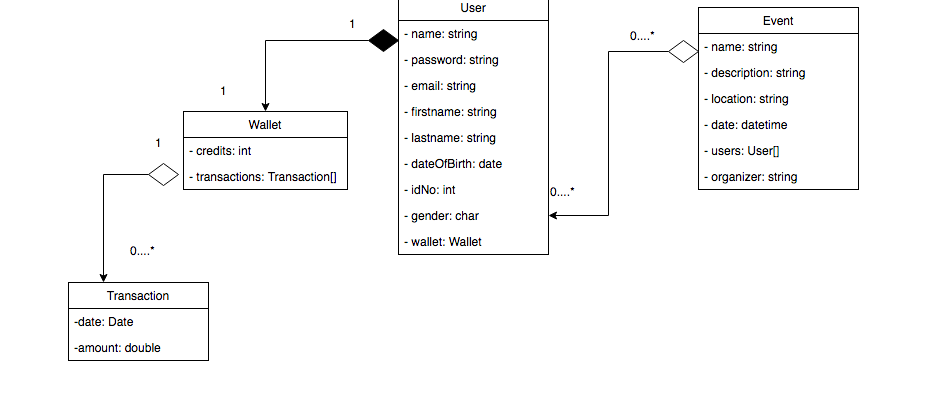
\includegraphics[scale=0.4]{Domain}
	\section{System Architecture}
	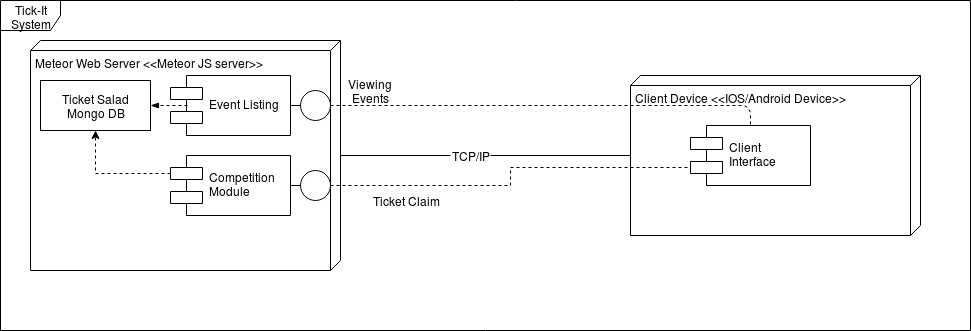
\includegraphics[scale=0.4]{Architecture}
	\newline
	The architecture used in the Ticket Salad application is client server. The system runs it's main database functions on a central server along with certain server functions which can then be accessed by the client device in order to verify data used for the application which runs on the client device.
	\section{Use Cases}
	
	
	\subsection{Logging in}
	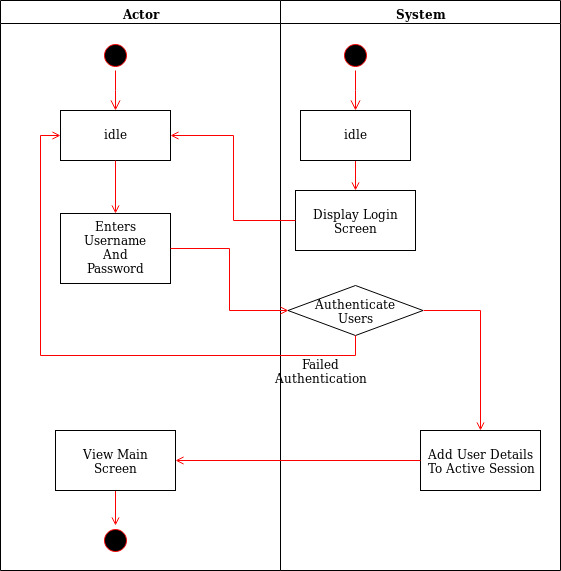
\includegraphics[scale=0.8]{Login.jpg}
	\subsection{Display Main screen}
	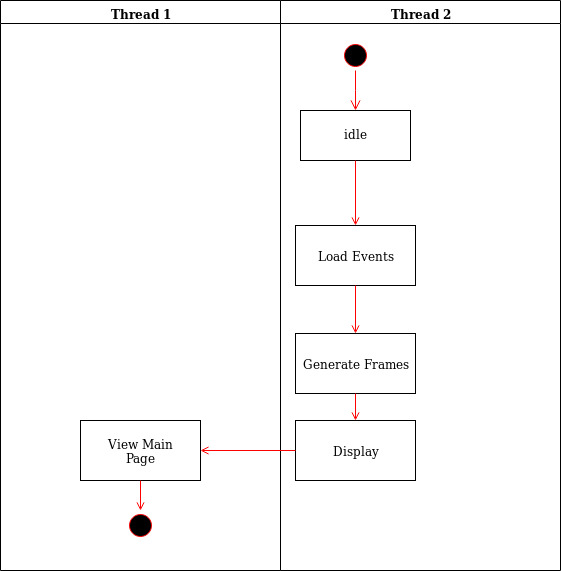
\includegraphics[scale=0.8]{Display}
	\subsection{Event Bidding}
	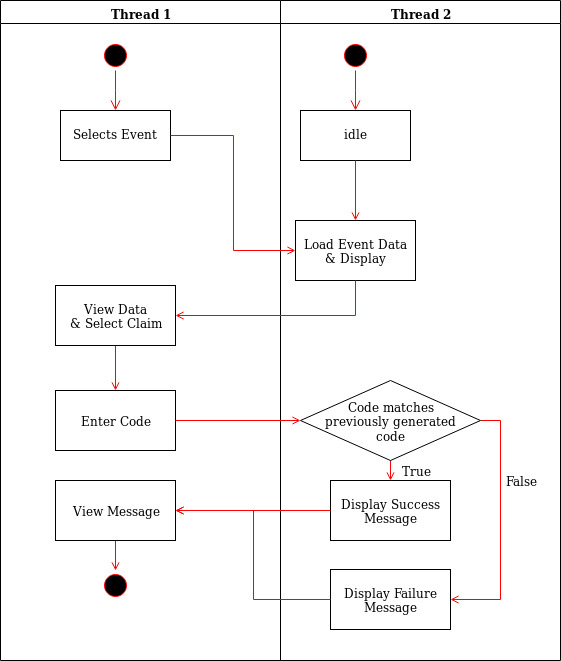
\includegraphics[scale=0.8]{Bid}
	
	
	
	
\end{document}